\documentclass[12pt]{book}
\usepackage[utf8]{inputenc}
\usepackage{amsmath, amssymb, amsfonts, amsthm}
\usepackage{bbm}
\usepackage{url}
\usepackage{geometry}
 \geometry{
 a4paper,
 left=20mm,
 right=20mm
 }

\linespread{1.1}
\usepackage{soul} % For strikethrough

\usepackage{pgfplots}
\pgfplotsset{compat=newest}
\usepackage{subfigure}


\usepackage{mathtools}
\mathtoolsset{showonlyrefs}

\usepackage{xcolor}
\definecolor{linkcolour}{rgb}{0,0.2,0.6}

\usepackage{hyperref}
\hypersetup{colorlinks,breaklinks,urlcolor=linkcolour, linkcolor=linkcolour}

\renewcommand{\iff}{\Longleftrightarrow}

\newtheorem{theorem}{Theorem}[chapter]
\newtheorem{proposition}[theorem]{Proposition}
\newtheorem{corollary}[theorem]{Corollary}
\newtheorem{lemma}[theorem]{Lemma}

\theoremstyle{definition}
\newtheorem{definition}{Definition}[chapter]

\theoremstyle{remark}
\newtheorem{ex}{Example}[chapter]
\newtheorem{remark}[theorem]{Remark}

\newcommand\numberthis{\addtocounter{equation}{1}\tag{\theequation}} % to number specific equations

\usepackage{enumitem}
\setenumerate[1]{label=(\roman*)}

\title{Nonlinear Dynamics and Chaos}
\author{Prof. George Haller\\ Transcription: Trevor Winstral}
\date{2022}
\setcounter{chapter}{-1}

\begin{document}
\maketitle
\tableofcontents 
\newpage

\chapter{Introduction}
First we shall introduce the most important characters in our following exploration. The ideas and definitions here will be recurring regularly as we examine them from different perspectives and using different tools. The content covered by this course can be found in the following books. For further details on some of the results, we recommend consulting these.
\begin{itemize}
	\item J. Guckenheimer \& P. Holmes, Nonlinear Oscillations, Dynamical Systems and Bifurcations of Vector Fields,
	\item F. Verhulst, Nonlinear Differential Equations and Dynamical Systems,
	\item V. I. Arnold, Ordinary Differential Equations,
	\item S. Strogatz, Nonlinear Dynamics and Chaos.
\end{itemize}


\begin{definition}[Dynamical System (DS)]
	A triple $(P,E, \mathcal{F})$, with
	\begin{itemize}
		\item $P :$ the phase space for the dynamical variable ${x} \in P$,
		\item  $E:$ base space of the evolutionary variable (e.g. time) $t \in E$,
		\item $\mathcal{F}: $ the evolution rule (deterministic) which defines the transition from one state to the next.
\end{itemize}
\end{definition}
The two main types of evolutionary variable spaces are
\begin{enumerate}
	\item Discrete dynamical systems (DDS) $t\in E=\mathbb{Z}$ with trajectory $\{ {x}_0,  {x}_1, \ldots\}$,
	\item Continuous dynamical systems (CDS) $t\in E=\mathbb{R}$ with trajectory $\{ {x}_t\}_{t \in \mathbb{R}}$.
\end{enumerate}
Corresponding to these there are various types of evolution rules
\begin{enumerate}
	\item In a DDS we have iterated mappings 
	\begin{align}
		\boxed{ {x}_{n+1} = F( {x}_n , n).}	
	\end{align}
	If there is no explicit dependence on $n$, i.e. $\frac{\partial F}{\partial n} = 0$, then 
	\begin{align}
		\boxed{  {x}_{n+1} F( {x}_n) = F(F( {x}_{n-1})) = \underbrace{F \circ \ldots \circ F}_{n+1 \textrm{ times} }( {x}_0) = F^{n+1}( {x}_0).}
	\end{align}
\begin{ex}[Cobweb diagram of a one-dimensional DDSs]
	In such cases and in one-dimensional problems, a simple way to analyze the behavior of the system is the so-called \textit{cobweb} diagram. We may plot $x_{n+1}$ as a function of $x_{n}$, as demonstrated in Fig. \ref{fig:cobweb}. The image of an initial condition $x_0$ lies on the graph at $x_{n+1}=F(x_0)$. We can also compute the next iterate by horizontally projecting the point $(x_0, F(x_0))$ to the diagonal line defined by $x_{n+1}= x_n$. Following the porjection of this point to the horizontal axis $(x_n)$ we find the intersection with the graph at the point $(x_1, F(x_1))$. It follows that fixed points on the cobweb diagram correspond to the intersection of the graph of $F$ with the diagonal line $x_{n+1}= x_n$.
	\begin{figure}[h!]
	\centering
	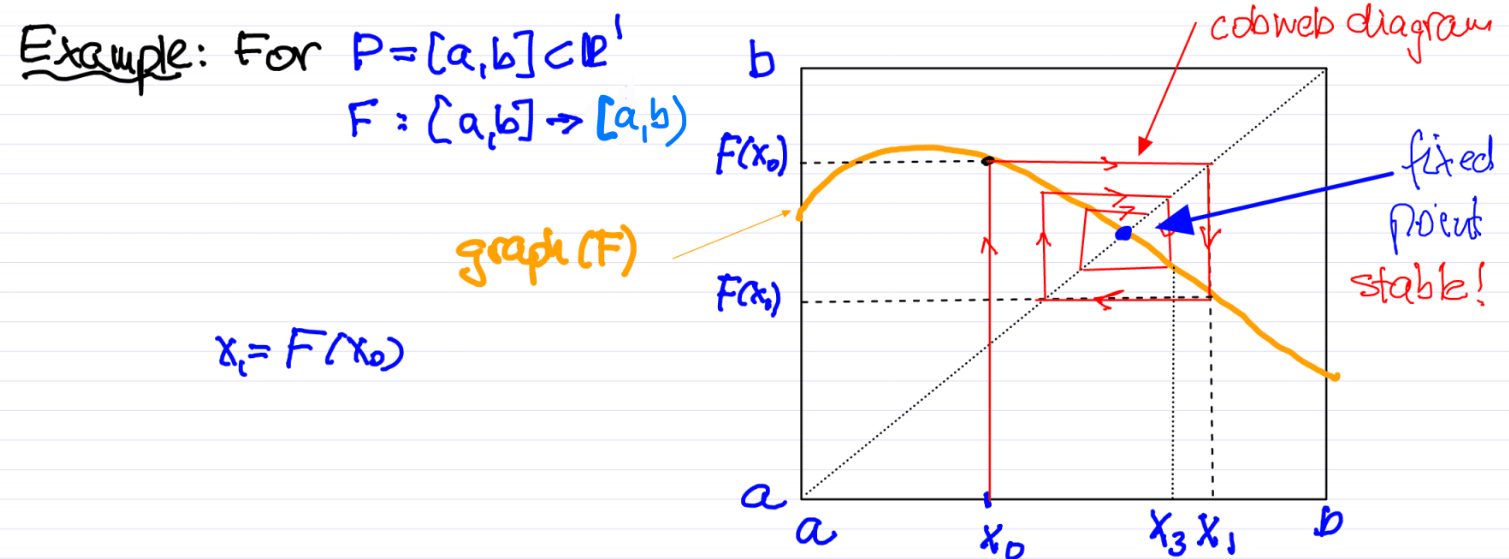
\includegraphics[width = \textwidth]{figures/intro/1DDS.png}
	\caption{Analysis of a one-dimensional system defined on the interval $x\in [a,b]$ using the cobweb diagram} \label{fig:cobweb}
\end{figure}
\end{ex}

\item In a CDS we have a first order system of ordinary differential equations (ODE)
	\begin{align}
		\boxed{
			\dot{ {x}} = f( {x},t)
		}
	\end{align}
	for $ {x}\in P$ and $t \in E$. This yields the initial value problem (IVP):
	\begin{align}
		\begin{dcases}
			\dot{ {x}} = f( {x},t) \\
			 {x}(t_0) =  {x}_0
		\end{dcases}
	\end{align}
	Assuming there exists a unique solution $\varphi(t; t_0,  {x}_0)$ with $\dot{\varphi} = f(\phi,t)$ and $\varphi(t_0)=  {x}_0$, then the following flow map is well defined
	\begin{align}
		\boxed{
		F_{t_0}^{t}( {x}_0) := \varphi(t; t_0,  {x}_0).}
	\end{align}

Geometrically, this solution can be viewed as a trajectory in phase space (cf. Fig. \ref{fig:cds_traj}).
	\begin{figure}[h!]
	\centering
	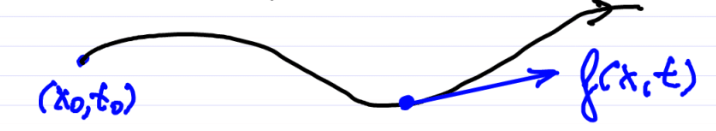
\includegraphics[width = 0.8\textwidth]{figures/intro/2CDS.png}
	\caption{Trajectory of a continuous dynamical system. The RHS is given by f(x,t), which is the tangent vector to this curve at the point $x$ at time $t$.} \label{fig:cds_traj}
	\end{figure}
	
	Such an $F_{t_0}^{t}$ has the properties
	\begin{enumerate}
		\item $F_{t_0}^{t}$ is as smooth as $f( {x},t)$,
		\item $F_{t_0}^{t_0} = I$ and $F_{t_0}^{t_2} = F_{t_1}^{t_2} \circ F_{t_0}^{t_1}$,
		\item $\left(F_{t_0}^{t}\right)^{-1} = F_{t}^{t_0}$ exists and is smooth.
\end{enumerate}
Properties (a) and (b) together are called the group property. A special case of continuous dynamical systems is the autonomous system.
\begin{align}
	\boxed{\dot{ {x}} = f( {x}).}	
\end{align}
The autonomy of a system implies
\begin{align}
	 {x}(s,t_0,  {x}_0) =  {x}(\underbrace{s-t_0}_{t}, 0,  {x}_0) \stackrel{!}{=}  {x}(t, {x}_0).
\end{align}
The induced flow map in this case is the one-parameter family of maps
\begin{align}
	\boxed{ F^{t} = F_{0}^{t}:  {x}_0 \mapsto  {x}(t, {x}_0).}
\end{align}
\end{enumerate}
\begin{ex}[Logisitic Equation]
	For a resource-limited population, we have the following dynamical system for $a> 0$, $b> 0$, and the population $x\in \mathbb{R}_+ \cup \{0\}$
	\begin{align}
		\dot{x} = ax(b-x).
	\end{align}
	In this case we have $E=\mathbb{R}$ and $\mathcal{F} = \{F^{t}\}_{t=-\infty }^{+\infty }$. This system has globally existing unique solutions (see later). We may analyze the behavior of this system by plotting $\dot{x}$ as a function of $x$, analogously to the cobweb diagram. This is demonstrated in Fig. \ref{fig:cds_analysis}. At $x$ values, where $\dot{x}$ is positive $x(t)$ is growing, while at negative values it is decreasing. This means, that fixed points, at which $x(t)=$ const. correspond to intersections of the graphs with the horizontal axis.
	\begin{figure}[h!]
		\centering
		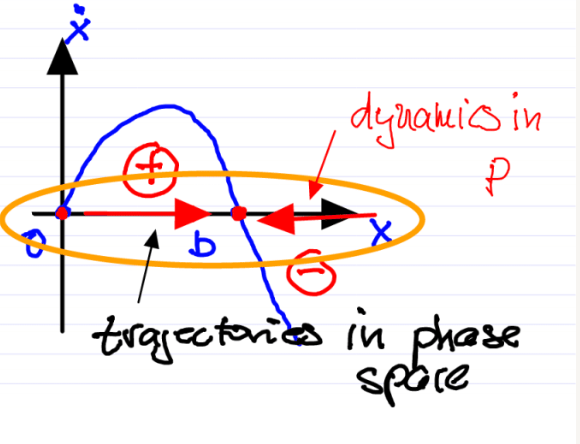
\includegraphics[width=0.4\textwidth]{figures/intro/3RHS.png}	
		\hspace{0.05\textwidth}
		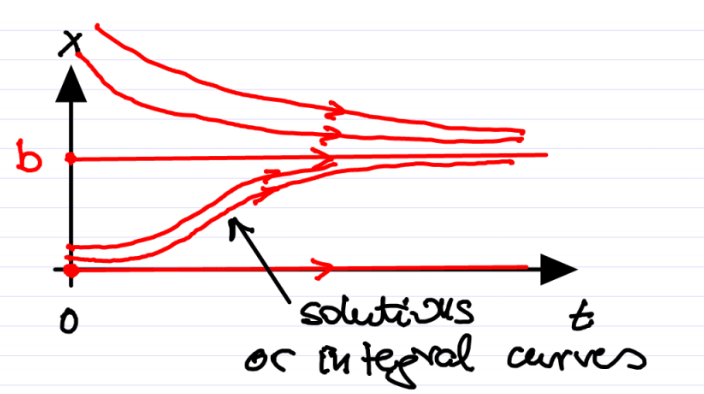
\includegraphics[width=0.4\textwidth]{figures/intro/4solutions.png}
		\caption{Left: Analysis of the right hand side. Right: Evolution in the extended phase space $P \times \mathbb{R}$.} \label{fig:cds_analysis}
	\end{figure}

\end{ex}

\begin{ex}[Pendulum]
Given the equation of motion
\begin{align}
	ml^2 \ddot{\varphi} = -mgl \sin(\varphi).
\end{align}
We let $ x_1 = \varphi$ and $ {x}_2 =\dot{\varphi}$ to transform into the first-order ODE form
\begin{align}
	\begin{dcases}
	\dot{x}_1 = x_2 \\
\dot{x}_2 = - \frac{g}{l} \sin (x_1).
	\end{dcases}
\end{align}
Thus we have 
\begin{align}
 {x} = 
\begin{pmatrix}
	x_1 \\ x_2
\end{pmatrix}; \quad
f( {x}) = 
\begin{pmatrix}
	x_2 \\ - \frac{g}{l}\sin(x_1)	
\end{pmatrix}.
\end{align}
Qualitative analysis gives the following facts
\begin{itemize}
	\item $(x_1, x_2) = (0,0)$ and $(x_1, x_2) = (\pi , 0)$ are zeros of $f$.
	\item Energy is conserved, hence both small and large amplitude oscillations are expected.
	\item The function $f(x)$ has symmetries: it is invariant under the transformation $(x_1, x_2, t) \mapsto (x_1, -x_2, -t)$ and $(x_1, x_2, t) \mapsto (-x_1, x_2, -t)$. See the left panel of Fig. \ref{fig:pendulum_symm+traj}.
\end{itemize}
\begin{figure}[h!]
	\centering
	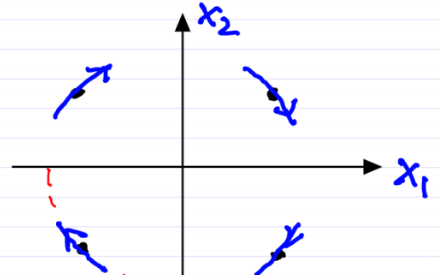
\includegraphics[width=0.4\textwidth]{figures/intro/6pendulum_symmetries.png}
	\hspace{0.05\textwidth}
	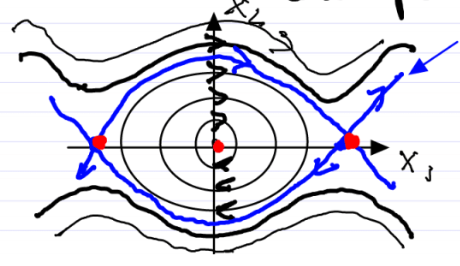
\includegraphics[width=0.4\textwidth]{figures/intro/5pendulum.png}
	\caption{Left: The symmetries of the dynamical system. Right: Phase portrait of the pendulum. Red dots show the fixed points, while the blue trajectories make up the separatrix.} \label{fig:pendulum_symm+traj}
\end{figure}
\begin{definition}
	A separatrix is a boundary (i.e. a codimension-1 surface) in phase space which separates regions of qualitatively different behaviors. In practice, it is unobservable by itself and connects different fixed points. The separatrix of the pendulum is shown in the right panel of Fig. 4.
\end{definition}

\end{ex}

\begin{ex}[Exploit geometry of phase space for analysis]
	Consider two cities, $A$ and $B$. The two cities are connected by two roads, denoted by the blue and green curves of the left panel of Fig. \ref{fig:two_cities}. We assume that travelling on the two roads, it is possible for two bikes to make it from $A$ to $B$ without ever being further away from each other than a distance $d<D$.

Assume two trucks are trying to make it between $A$ and $B$, on different roads in the opposite direction, carrying a load of width $D$. Given this information, can the trucks make it without hitting each other? We can view this problem as a continuous dynamical system with two coordinates $x_1$ and $x_2$ that parameterize the two routes between $A$ and $B$. This dynamical system is, in general, non autonomous.
	\begin{figure}[h!]
		\centering
		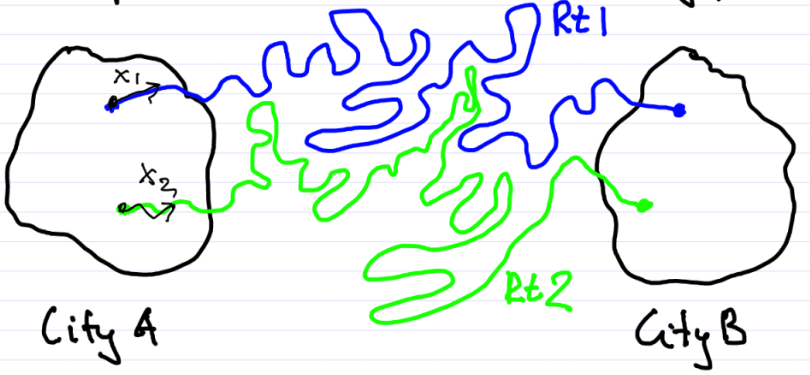
\includegraphics[width=0.5\textwidth]{figures/intro/7routes.png}
		\hspace{0.05\textwidth}
		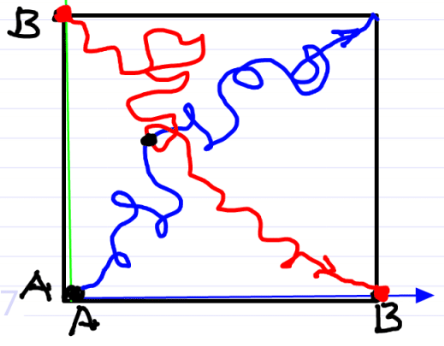
\includegraphics[width=0.3\textwidth]{figures/intro/8truck_geometry.png}
		\caption{Left: An example of the two bike routes. Right: Blue represents the trajectory of the two bikes, red represents the trajectory of the two trucks.} \label{fig:two_cities}
	\end{figure}

	The right panel of Fig \ref{fig:two_cities} shows the trajectories of the two trucks and the two bikes in phase space. The two trajectories must intersect by continuity, thus at that point the trucks must be at the same positions as the bikes, implying they are within distance $D$. Therefore the trucks must crash!	
\end{ex}



\newpage

\chapter{Fundamentals}
\section{Existence and uniqueness of solutions}
Consider  
\begin{align}
\begin{dcases}
	\dot{x} = f(x,t); & x \in \mathbb{R}^{n} \\
	x(t_0) = x_0
\end{dcases}.
\end{align}
Does this initial value problem have a unique solution? We have the following theorems to help us answer that question.
\begin{theorem}[Peano]
	\label{thm:Peano}
	If $f\in C^0$ near $(x_0, t_0)$, then there exists a local solution $\varphi(t)$, i.e., 
\begin{align}
	\dot{\varphi}(t) = f(\varphi(t), t), \varphi(t_0) = x_0;\ \forall  t\in (t_0 - \epsilon, t_0 + \epsilon);\ 0<  \epsilon \ll 1.
\end{align}
\end{theorem}
\begin{ex}[Free falling mass]
	We have that the total energy is conserved
	\begin{align}
		\frac{1}{2} m \dot{x}^2 = mg(x-x_0).
	\end{align}
This implies that
\begin{align}
	\begin{dcases}
		\dot{x} = \sqrt{2g(x-x_0)} \\
		x(0) = x_0
	\end{dcases}
\end{align}
on the set $P = \{ x \in \mathbb{R}:\ x \geq x_0\}$. Therefore we have that $f\in C^0$ in phase space, so by Peano's theorem (cf. \ref{thm:Peano}), there exists a local solution.
	\begin{figure}[h]
		\centering
		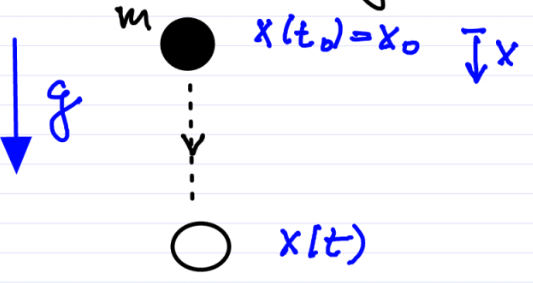
\includegraphics[width=0.4\textwidth]{figures/ch1/1freefall.png}
	\end{figure}
	The solution is actually $x(t) = x_0 + \frac{g}{2}(t-t_0)^2$, however $x(t) = x_0$ is also a solution to the IVP, therefore we do not have a unique solution. Physically there exists a solution, but this IVP was derived from a heuristic energy-principle, not from Newton's laws, which are not equivalent.
\end{ex}
\begin{definition}
A function is called locally Lipschitz around $x_0$ if there exists an open set $U_{x_0}$ and $L>0$ such that for all $x,y \in U_{x_0}$
\begin{align}
	\boxed{\left| f(y,t) - f(x,t)\right| \leq L |y - x|.}
\end{align}
\end{definition}

\begin{ex}[Lipschitz functions]
	Here we have an example of a Lipschitz and a non-Lipschitz function around $x_0$.
	\begin{figure}[h]
		\centering
		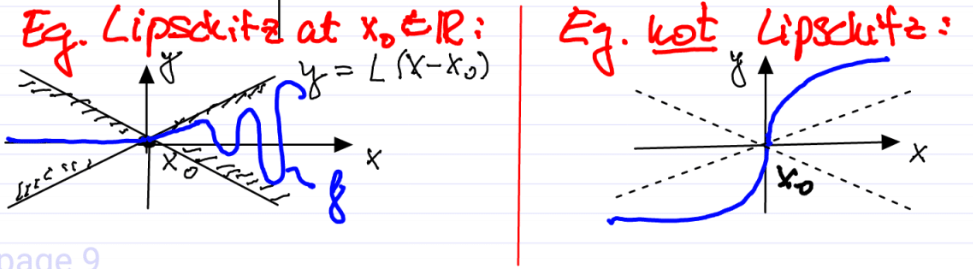
\includegraphics[width=0.8\textwidth]{figures/ch1/2lipschitz.png}
	\end{figure}
\end{ex}

\begin{theorem}[Picard]
	Assume 
	\begin{enumerate}
		\item  $f \in C^0$ in $t$ near $(t_0, x_0)$,
		\item $f$ is locally Lipschitz in $x$ near $(t_0, x_0)$.
	\end{enumerate}
	Then there exists a unique local solution to the IVP. The proof from Arnold's ODE. 	
\end{theorem}
\textbf{Note} $f$ is $C^1$ $\implies$ $f $ is Lipschitz $\implies $ $f$ is $C^0$.
\begin{ex}[Free falling mass revisted]
	We check if $f$ is Lipschitz.
	\begin{align}
		\frac{| f(x) - f(x_0) |}{|x-x_0|} = \frac{\sqrt{2g}}{\sqrt{|x-x_0|}} \not< L | x - x_0|.
	\end{align}
Thus $f$ is not Lipschitz near $x_0$.	
\end{ex}

\section{Geometric consequences of uniqueness}
If the solution is unique, we have a few facts that can be derived from the geometric point of view.
\begin{enumerate}
	\item The trajectories of autonomous systems cannot intersect. Note that fixed points do not violate this (e.g. pendulum equations).
		\begin{figure}[h]
			\centering
			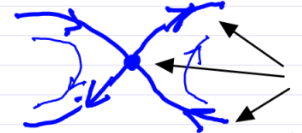
\includegraphics[width=0.3\textwidth]{figures/ch1/3pendulum_trajectories.png}
			\caption{The phase portrait of the pendulum. Trajectories do not intersect since each arrow is pointing at separate trajectories.}
		\end{figure}
		
	\item For non-autonomous systems, intersections in phase space are possible. In which case we can extend the phase space in order to get an autonomous system where there cannot be any intersections.
		\begin{align}
			X = 
			\begin{pmatrix}
				x \\ t
			\end{pmatrix},\
			F(X) = 
			\begin{pmatrix}
				f(x,t) \\ 1
			\end{pmatrix};\
			\dot{X} = F(X).
		\end{align}
		\begin{figure}[h]
			\centering
			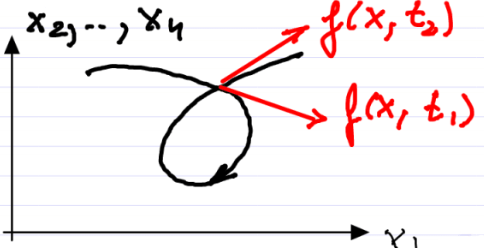
\includegraphics[width=0.4\textwidth]{figures/ch1/4intersecting_trajectories.png}
			\hspace{0.05\textwidth}
			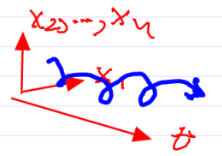
\includegraphics[width=0.3\textwidth]{figures/ch1/5extended_space.png}
			\caption{Left: Intersecting trajectories in phase space for a non-autonomous system. Right: The same trajectory in the extended phase space, without intersections.}
		\end{figure}
\end{enumerate}

\section{Local vs global existence}
\begin{ex}[Exploding solution]
	\begin{align}
		\begin{dcases}
			\dot{x} = x^2 \\
			x(t_0) = 1.
		\end{dcases}
	\end{align}
	Integrating yields the solution $x(t) = \frac{1}{1 - (t-t_0)}$. This solution blows up at $t_{\infty }=t_0 + 1$, therefore the solution is only local.	
\begin{figure}[h]
\centering	
\begin{tikzpicture}
	\begin{axis}
		[xmin=0, xmax=2.5, ymin=0.5, ymax=3, domain = 1:1.9, xlabel=$t$, ylabel=$x(t)$, xtick=\empty, ytick=\empty]
		\addplot[color=black] {1/(2-x)};
		\addplot[color=black, dashed] coordinates {(1.7,0.5) (1.7,3.1)} node[pos=0, above right] {$t_{\infty }$};
		\addplot[color=black, dashed] coordinates {(1,0.5) (1,1)} node[pos=0, above right] {$t_{0}$};
		\addplot[color=black, dashed] coordinates {(0,1) (1,1)} node[pos=0, above right] {$x_{0}$};
	\end{axis}
\end{tikzpicture}
\end{figure}
\end{ex}

\begin{theorem}[Continuation of solution]
	If a local solutions cannot be continued to to a time $T$, then we must have
	\begin{align}
		\boxed{\lim_{t\to T} |x(t)|= \infty.}
	\end{align}
The proof from Arnold's ODE.	
\end{theorem}

\begin{ex}[Coupled Pendulum System]
	We set $x_1 = \varphi_1,\ x_2 = \dot{\varphi_1},\ x_3 = \varphi_2,\ x_4=\dot{\varphi_2} $ and get the following equation of motion
\begin{align}
	\begin{dcases}
		\dot{x}_1 = x_2 \\ \dot{x}_2 = \ldots \\ \dot{x}_3 = x_4 \\ \dot{x}_4 = \ldots
	\end{dcases}
\end{align}
The RHS is smooth, therefore there exists a unique local solution to any IVP.
\begin{figure}[h]
	\centering
	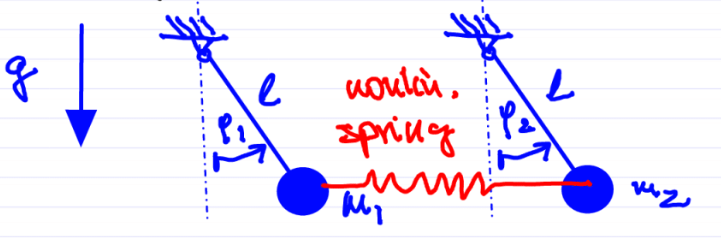
\includegraphics[width=0.6\textwidth]{figures/ch1/6coupled_pendulum.png}
	\caption{Physical setup of the coupled pendulum with a nonlinear spring.}
\end{figure}
The phase space is given by 
\begin{align}
	P = \{x:\ x_1 \in S^1,\ x_2 \in \mathbb{R},\ x_3 \in S^1,\ x_4 \in \mathbb{R} \} = S^1 \times \mathbb{R}\times S^1 \times \mathbb{R}.
\end{align}
Where $S^1$ is the 1 dimensional sphere (i.e. a circle). With this space we know that $|x_1|$ and $|x_3|$ are bounded. Due to energy being conserved we have
\begin{align}
	E &= T+V = \frac{1}{2}m_1 l_1 x_2^2 + \frac{1}{2}m_2 l_2 x_4^2 + \underbrace{V(x_1, x_3)}_{\geq 0}\\
	E &= E_0 =  \textrm{constant} \geq 0.
\end{align}
Hence $|x_2|$ and $|x_4|$ are also bounded, therefore all solutions exist globally.
\end{ex}
\begin{definition}
	A linear system is one such that for $x\in \mathbb{R}^{n},\ A(t) \in \mathbb{R}^{n\times n}$ and $A\in C^0$ 
	\begin{align}
		\boxed{\dot{x} = A(t) x.}
	\end{align}
\end{definition}

\begin{remark}[]
	Note that  $S = \frac{1}{2}(A + A^T)$ is symmetric (i.e. $S = S^T)$ and $\Omega = \frac{1}{2}(A - A^T)$ is skew symmetric (i.e. $\Omega = -\Omega^T$). Furthermore the eigenvalues of $S$, $\lambda_i$, are all real and their respective eigenvectors, $e_i$, are orthogonal.
\end{remark}

\begin{ex}[Global existence in linear systems]
\begin{align}
	\langle x, \dot{x} \rangle &= \frac{1}{2} \frac{d}{dt} |x(t)|^2 = \langle x, A(t) x\rangle = \langle x, (S(t) + \Omega(t) ) x \rangle \\
				   &= \langle x, S(t) x \rangle + \underbrace{\langle x, \Omega(t) x \rangle}_{=0} \stackrel{(*)}{=} 
				   \sum_{i=1}^{n} \lambda_i(t) x_i^2 \\
				   &\leq \lambda_{ \textrm{max} }(t) \sum_{i=1}^{n} x_i^2 = \lambda _{ \textrm{max} }(t) | x(t)|^2.
\end{align}
Where in $(*)$ we used that $x = \sum_{i=1}^{n} x_i e_i $ with $|e_i|=1$ and $e_i \perp e_j$ for all $i \neq j$. Thus we get
\begin{align}
	\frac{\frac{1}{2}\frac{d}{dt}|x(t)|^2}{|x(t)|^2} \leq \lambda_{ \textrm{max} }(t) 
	\implies \int_{t_0}^{t} \log \left( \frac{|x(s)|^2}{|x(t_0)|^2} \right) ds \leq \lambda _{ \textrm{max} }(s) ds.
\end{align}
By exponentiating both sides, we obtain
\begin{align}
\boxed{ |x(t)| \leq |x(t_0) | \exp\left(\int_{t_0}^{t} \lambda_{ \textrm{max} }(s)ds\right).}
\end{align}
Therefore, by the continuation theorem, global solutions exist as long as $\int_{t_0}^{t} \lambda_{ \textrm{max} }(s) ds < \infty $.
\end{ex}

\section{Dependence on initial conditions}
Given the IVP
\begin{align}
	\begin{dcases}
	\dot{x} = f(x,t) \\ x(t_0) = x_0.
	\end{dcases}
\end{align}
With $x \in \mathbb{R}^{n}$ and $f\in C^r$ for some $r\geq 1$, we have the solution $x(t; t_0, x_0)$.
\textbf{Question} How does the solution depend on initial data?
But first, why do we care about this? Because we robust solutions with respect to errors and uncertainties in the initial data.
\begin{theorem}[]
	If $f \in C^r$ for $r\geq 1$ then $x(t; t_0, x_0)$ is $C^r$ in $(t_0, x_0)$. Proof in Arnold's ODE.
\end{theorem}

The geometric meaning of this is that for $U \subset P \subset \mathbb{R}^{n}$ we have that $F_{t_0}^{t}(U)$ is a smooth deformation of $U$.
\begin{figure}[h]
	\centering
	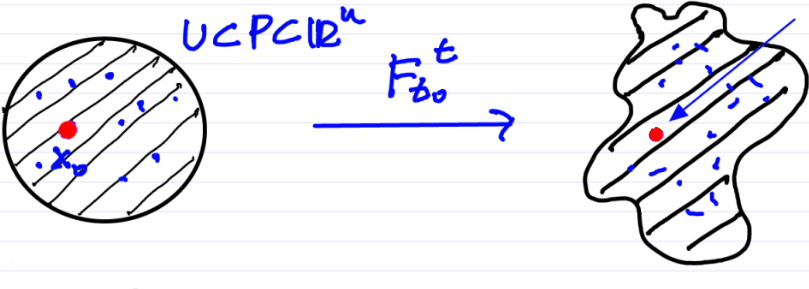
\includegraphics[width=0.7\textwidth]{figures/ch1/7smooth_transform.png}
	\caption{The smooth transformation of $U$. The red point on the right it $F _{t_0}^t(x_0)$, i.e. the image of $x_0$ through the evolution operator.}
\end{figure}
It turns out $\left(F_{t_0}^{t}\right)^{-1} = F_{t}^{t_0}$ is also $C^r$, hence we have that $F_{t_0}^{t}$ is a diffeomorphism. 

Now, how can we compute the Jacobian of the flow map $\frac{\partial x(t; t_0, x_0)}{ \partial x_0} = DF _{t_0}^{t}(x_0)$? We will use the IVP.
\begin{align}
	\frac{d}{dt}\frac{\partial x}{\partial x_0} = D_x f(x(t; t_0, x_0), t) \frac{\partial x}{\partial x_0}.
\end{align}
The flow gradient satisfies the IVP
\begin{align}
	\frac{d}{dt}\left[ DF_{t_0}^{t}(x_0)\right] &= D_{x}f(F_{t_0}^{t}(x_0), t) DF_{t_0}^{t}(x_0) \\
	DF_{t_0}^{t_0}(x_0) &= I.
\end{align}
This gives us the equation of variations (linear, non-autonomous)
\begin{align}
	\begin{dcases}
		\dot{M} = D_x f(x(t; t_0, x_0)) M \\ M(t_0) = I.
	\end{dcases}
\end{align}

\begin{ex}[Locations of extreme deformation in phase space]
	We define 
	\begin{align}
		\xi(t) &:= \tilde{x}(t) - x(t) = x(t; t_0, \tilde{x_0}) - x(t; t_0, x_0)\\
		       &= x(t; t_0, x_0) + \frac{\partial x}{\partial x_0}(t; t_0, x_0)\xi_0 + \mathcal{O}(|\xi_0|^2) - x(t; t_0, x_0) \\
		       &= DF_{t_0}^{t}(x_0)\xi_0 + \mathcal{O}(|\xi_0|^2).
	\end{align}
	Where we used the Taylor expansion and assume the perturbation to $x_0$ is small, i.e. $|\xi_0| \ll 1$.
	\begin{figure}[h]
		\centering
		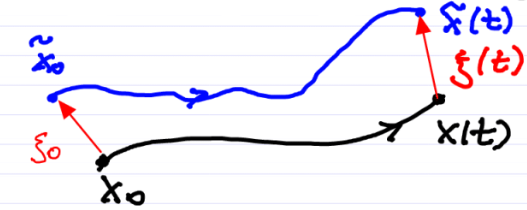
\includegraphics[width=0.5\textwidth]{figures/ch1/8dispersion.png}
	\end{figure}
	Therefore we have
	\begin{align}
		|\xi(t)|^2 &= \langle DF_{t_0}^{t}(x_0) \xi_0, DF_{t_0}^{t}(x_0)\xi_0 \rangle + \mathcal{O}(|\xi_0|^3) \\
			   &= \langle \xi_0, \underbrace{\left[ DF_{t_0}^{t}(x_0) \right]^T DF_{t_0}^{t}(x_0)}_{=: C_{t_0}^{t}(x_0)} \xi_0 \rangle + \mathcal{O}(|\xi_0|^3).
	\end{align}
	$C_{t_0}^{t}(x_0)$ is known as the Cauchy-Green strain tensor (field of $n\times n$ symmetric matrices).
	Therefore the largest possible deformation is
	\begin{align}
		\max_{x_0, xi_0} \frac{|\xi(t)|^2}{|\xi_0|^2} = \max_{x_0, \xi_0}\frac{\langle \xi_0, C_{t_0}^{t}(x_0) \xi_0 \rangle}{|\xi_0|^2} = \max_{x_0} \lambda_{n}(x_0).
	\end{align}
	Where we used that $C_{t_0}^{t}$ is positive definite in the last equality, and that $\lambda_n(x_0)$ is the largest eigenvalue of $C_{t_0}^{t}(x_0)$. We typically have exponential growth.	
\end{ex}
\begin{definition}
	The finite-time Lyapunov exponent is defined as
	\begin{align}
		\boxed{ \textrm{FTLE} _{t_0}^{t}(x_0) := \frac{1}{2(t-t_0)} \log(\lambda_n(x_0)).}
	\end{align}
\end{definition}
The FTLE is a diagnostic quantity for Lagrangian Coherent Structure (LCS), i.e. influential surfaces governing the evolution in $P$.
\begin{figure}[h]
	\centering
	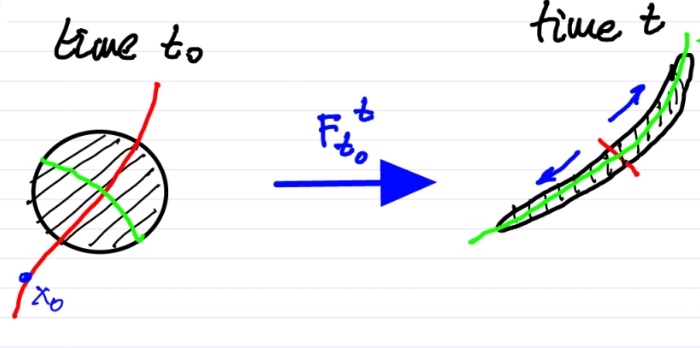
\includegraphics[width=0.6\textwidth]{figures/ch1/9deformation.png}
	\caption{On the left the red ridge represents large values of $ \textrm{FTLE} _{t_0}^{t}$, on the right the green ridge the high values of $ \textrm{FTLE} _{t}^{t_0}$.}
\end{figure}
\begin{figure}[h]
	\centering
	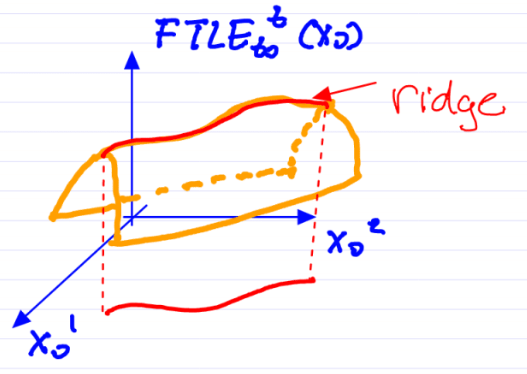
\includegraphics[width=0.4\textwidth]{figures/ch1/10ridge_projection}
	\caption{The projection of the FTLE ridge onto the initial value space.}
\end{figure}

The ridges of $ \textrm{FTLE} _{t_0}^{t}$ are the repelling LCS, meanwhile the ridges of $ \textrm{FTLE} _{t}^{t_0}$ are the attracting LCS. Now we are left with the problem of computing $F_{t_0}^{t}(x_0)$. Recall that analytically we start with $F_{t_0}^{t}(x_0)$ and use this to calculate $DF_{t_0}^{t}(x_0)$. From here we can find $C_{t_0}^{t}(x_0)$, giving us $\lambda_n(x_0)$ and thereby the FTLE. We know approximate this process numerically.
\begin{enumerate}
	\item Define an initial $M\times N$ grid of initial data $x_0(i,j) \in \mathbb{R}^2$.
	\item Launch trajectories numerically from grid points to obtain a discrete approximation of $F_{t_0}^{t}(x_0)$ as $F_{t_0}^{t}(x_0(i,j))$.
	\item Use finite differencing to approximate $DF_{t_0}^{t}(x_0(i,j)).$
\end{enumerate}

\begin{ex}[Double gyre model using FTLE]
We have the stream function
\begin{align}
	\Psi(x,y) = -\sin(\pi x) \sin(\pi y).
\end{align}
This gives the fluid velocity field
\begin{align}
	V = 
	\begin{dcases}
		\dot{x} = \frac{\partial \Psi}{\partial y} \\
		\dot{y} = - \frac{\partial \Psi}{\partial x}.
	\end{dcases}
\end{align}
\begin{remark}[]
This is an example of a Hamiltonian system of $\Psi$ being the Hamiltonian $H$.
\end{remark}
For any autonomous Hamiltonian system we have that $H$ is constant along trajectories, we check
\begin{align}
	\frac{d}{dt}\Psi(x(t),y(t)) = \frac{\partial \Psi}{\partial x}\dot{x} + \frac{\partial \Psi}{\partial y}\dot{y} = 0.
\end{align}
So we have that trajectories are level curves of $\Psi(x,y)$. We can then derive the phase portrait from the level curves of $\Psi$. Further, we have that $\dot{x} = \frac{\partial \Psi}{\partial y} = - \pi \sin(\pi x) \cos(\pi y)$ which yields that $ \textrm{sign} (\dot{x}) = -  \textrm{sign} (\sin(\pi x))  \textrm{sign} (\cos(\pi y))$. Putting these together we can construct the contour plot with arrows.

\begin{figure}[h]
	\centering
	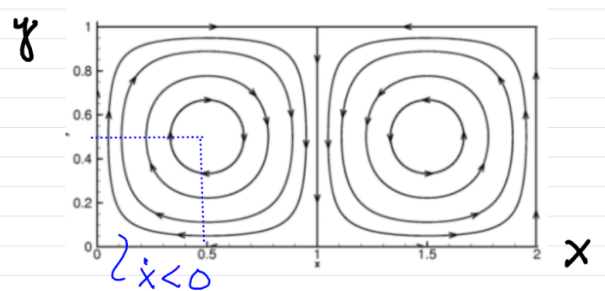
\includegraphics[width=0.5\textwidth]{figures/ch1/11contour_phase.png}
	\hspace{0.03\textwidth}
	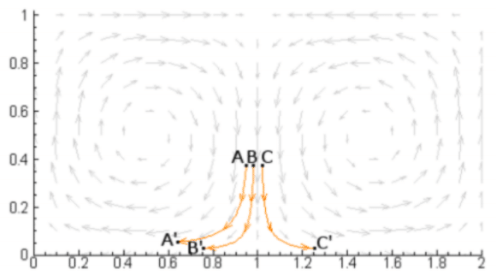
\includegraphics[width=0.45\textwidth]{figures/ch1/12ftle_exploration.png}
	\caption{}
	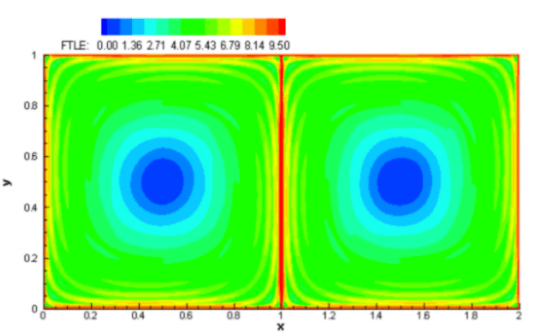
\includegraphics[width=0.5\textwidth]{figures/ch1/13ftle_final.png}
	\caption{Top left: The analytic phase plot. Top right: The exploration done to calculate FTLE. Bottom: The FTLE plot.}
\end{figure}
Figures here were taken from Shawn Shadden of UC Berkely.
\end{ex}

\begin{ex}[ABC flow]
	Let our dynamic system be defined as follows with $A,B,C \in \mathbb{R}$
\begin{align}
	\begin{dcases}
		\dot{x} = A \sin(z) + C \cos(y) \\
		\dot{y} = B \sin(x) + A \cos(z) \\
		\dot{z} = C \sin(y) + B \cos(x).
	\end{dcases}
\end{align}
We are looking for an exact solution of Euler's equation of inviscid fluids. We have an autonomous velocity field, which is known to generate chaotic fluid trajectories.
\begin{figure}[h]
	\centering
	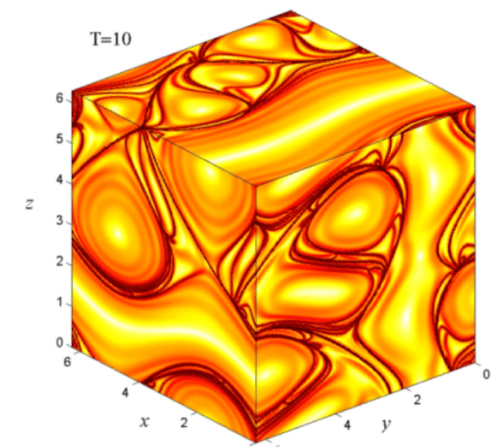
\includegraphics[width=0.4\textwidth]{figures/ch1/14fluid1.png}
	\hspace{0.03\textwidth}
	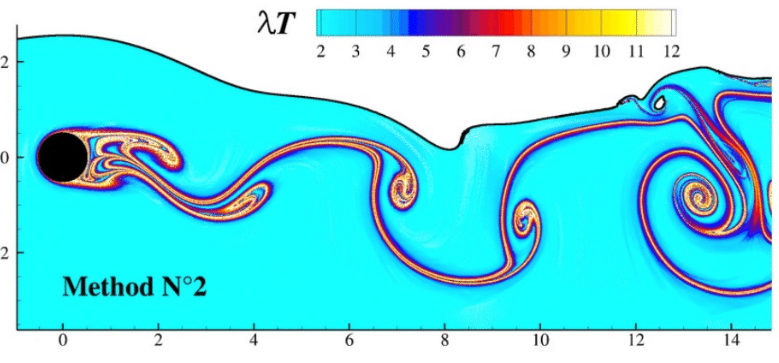
\includegraphics[width=0.55\textwidth]{figures/ch1/15vortex_shedding.png}
	\caption{Left: numerical results of dynamic system (Guckenheimer-Holmes Physica D, 2001). Right: vortex shedding behind a cylinder under a free surface (Sun et. al, 2016).}
\end{figure}
\end{ex}
\vfill
\section{Dependence on parameters}
We now have the IVP
\begin{align}
	\begin{dcases}
		\dot{x} = f(x,t, \mu ) \\ x(t_0) = x_0.
	\end{dcases}
\end{align}
With $x \in \mathbb{R}^{n},\ f\in C^r,\ r\geq 1$, therefore we have a solution $x(t; t_0, x_0, \mu ) \in C^r_{x_0}$.

\textbf{Question} How does the solution depend on $\mu $? 
\textbf{Why Care?} We would like robustness of solutions with respect to parameter changes or uncertainties in the model.
\begin{ex}[Perturbation Theory]
Given a weakly nonlinear oscillator
\begin{align}
	m \ddot{x} + c \dot{x} + kx = \epsilon f(x, \dot{x}, t),\ 0 \leq \epsilon \ll 1,\ x \in \mathbb{R}.
\end{align}
The usual approach is to seek solutions by expanding from known solution of the linear limit, i.e.
\begin{align}
	x_{\epsilon}(t) = \varphi_0(t) + \epsilon \varphi_1(t) + \epsilon^2 \varphi_2(t) + \ldots + \mathcal{O}(\epsilon^r).
\end{align}
If $x_{\epsilon}(t)$ is in $C^{r}_{\epsilon}$, we have $\varphi_1(t) = \left.\frac{\partial x_\epsilon(t)}{\partial \epsilon}\right|_{\epsilon =0}$ and $\varphi_2(t) = \left.\frac{\partial^2 x_\epsilon(t)}{\partial \epsilon^2}\right|_{\epsilon =0}$
\end{ex}

\textbf{Answer} Regularity with respect to $\mu $ actually follows from regularity with respect to $x_0$. Use the trick of extending the IVP with a dummy variable $\mu $ 
\begin{align}
	\begin{dcases}
		\dot{x} = f(x,t,u) \\ \dot{mu} = 0 \\ x(t_0) = x_0 \\ \mu (t_0) = mu_0.
	\end{dcases}
\end{align}
Thus with $X=
\begin{pmatrix}
	x \\ \mu 
\end{pmatrix}
\in \mathbb{R}^{n+p}$ and $F(X_0) = 
\begin{pmatrix}
	f \\ 0
\end{pmatrix};\ X_0 = 
\begin{pmatrix}
	x_0 \\ \mu _0
\end{pmatrix}
$. Therefore we have
\begin{align*}
	\begin{dcases}
		\dot{X} = F(X) \\ X(t_0) = X_0
	\end{dcases} \numberthis \label{eq:ivp_param}
\end{align*}
Applying the previous result on regularity with respect to $x_0$ to \eqref{eq:ivp_param}, we have that $f\in C^{r}_{x,\mu }$ implies that $X(t) \in C^{r}_{X_0}$ in turn implying that $x(t; t_0, x_0, \cdot) \in C^{r}_{\mu }$. The solution is as smooth in parameters as the RHS of the dynamic system.


\newpage

\end{document}

